\documentclass[12pt,a4paper,titlepage]{article}
%\usepackage[doublespacing]{setspace}
\usepackage[utf8]{inputenc}         %This is used for ASKII digits.
\usepackage{amsmath, amssymb}       %This is for mathematic statements,check"amath.colorado.edu/documentation/LaTex/Symbols.pdf"
\usepackage{amsfonts,mathrsfs}      %fonts~~
\usepackage{graphicx}               %This is for graph inserting.
\usepackage{paralist}               %Give me compact lists!!!!! 'compactitem' 'compactenum' 'compactdesc'
%\usepackage{bm}
\usepackage{caption2}                 %various kinds of bold texts.
\usepackage[top =2.54cm, bottom =2.54cm, left =3.18cm, right =3.18 cm]{geometry}
\usepackage{indentfirst}            %Indent the first letter
\usepackage{fancyhdr}               %Below is the head of the article.
\pagestyle{fancy}
\usepackage{booktabs}
\usepackage{makecell}
\usepackage{lastpage}
\lhead{Team \# 33131}
\rhead{Page \thepage{} of \pageref{LastPage}}
\cfoot{}
%\numberwithin{equation}{section}    %Numbering of the equations will be based on sections.
%\usepackage{amsthm}
%\theoremstyle{definition}
%\newtheorem{def}{Definition}  %Below set the theorem system.
%\theoremstyle{plain}
%\newtheorem{thm}[law]{Thm}
%\theoremstyle{remark}
%\newtheorem*{remark}{Remark}
\newcommand{\boldit}[1]{\textbf{\textit{#1}}}
\usepackage{float}
\usepackage{paralist}
\usepackage{url}

\begin{document}

\title{Integrated Management Model for Human Capital}
\date{}
\maketitle

\tableofcontents

\newpage

\section{Introduction}
\label{sec:introduction}

Considering the shortage of the talent, it's essential for companys to
retain good people and make them well-trained. However, current
situation is not satisfactory while many talents always tend to get a
good job via job-hopping, causing orgnizational churn in employees who
are closely connected to them.

ICM is facing such an issue that the churn rate reachs 18\%. The churn rate of middle managers even reaches twice as much as others. At present, the company only has 85\% of its positions occupied while HR is recruiting only 8\%-10\% of the vacancies due to limited resources. In addition, HR department hopes to place employees to suitable positions to maximize their talent. In order to simulate this situation and help to improve it, we build a human capital model based on Social Network
Analysis and Markov process.

There are several tasks we need to accomplish:

\begin{itemize}
\item Build a Human Capital network model of ICM's personnel situation.

\item Identify dynamic processes within the Human Capital network,
  which includes organizatinal churn and direct and indirect effects on
  the organization's productivity.

\item Analyze the organization's budget requirements over the next 2
  years.

\item Judge if ICM could sustain its 80\% full status for positions if
  the annual churn rate for all positions goes to 25\% and 35\%
  respectively. Calculate the costs of these higher turnover rates and
  describe the indirect effects of these high churn rates.

\item Assumes that there is no external recruiting and ICM promotes
  only qualified employees for the next two years. Simulate the impact
  of 30\% churn rate in both junior managers and experienced
  supervisors, if other churn values remain 18\%.

\item Connect our Human Capital network to other organizational
  network layers such as information flow, trust, influence, and
  friendship that the other offices of ICM are considering building.
\end{itemize}
\section{Variables and Descriptions}

Definitions of symbols employed in this section are listed in \textbf{Table
\ref{variable1}}, where all the subscripts with $t$ represent the
$t$-th month and all the subscripts with $i$ represent the employee
indexed by $i$:

\begin{table}
  \centering
  \begin{tabular}{l p{10cm}}
  \toprule[2pt]
  Variable & Description \\
  \midrule{}
  $i$            &Index of an employee \\
  $L_{i,t}$          &The level of $i$ \\
  $A_{ac_i,t}$       &The work achievement of $i$ \\
  $A_{ab_i,t}$         &The work ability of $i$ \\
  $A_{at_i,t}$        &The work attitude of $i$ \\
  $A_{po_i,t}$       &The potential of $i$ \\
  $A_{i,t}$          &The grade of $i$ \\
  $s_{ij,t}$        &The relation strength from $i$ to $j$ \\
  $a_{ij,t}$        &The influence caused by leader-member relation
                    between $i$ and $j$ \\
  $f_{ij,t}$        &The influence caused by friendship
                    between $i$ and $j$\\
  $c_{i,t}$        &The Clustering Coefficient of $i$ \\
  $p_{i,t}$           &Promotion probability of $i$\\
  $l_{i,t}$          &Churn probability of $i$ \\
  $prod_{i,t}$       &Productivity of $i$ \\
  $salary_{i,t}$     &Salary of $i$ \\
  $d_{i,t}$          &The work experience of $i$ \\
  $m_{ij}$           &The variable to reflect whether employee indexed
                       by $i$ is suitable for position indexed by $j$
                       \\
  $B_{ac_j}$       &The suitable work achievement of position indexed
                     by  $j$ \\
  $B_{ab_j}$       &The suitable work ability of position indexed by
                     $j$ \\
  $B_{at_j}$       &The suitable work attitude of position indexed by
                     $j$ \\
  $B_{po_j}$       &The suitable potential of position indexed by $j$
                     \\
  $N$ & The number of employees over the next two years \\
$p$ & The average productivity over the next two years \\
$r$ & The percentage of recruiting positions in ICM positions \\
$c$ & The current churn rate \\
$ra$ & The ratio of the churn rate between middle managers and the
       rest employees \\
  \bottomrule[2pt]
\end{tabular}
\caption{Variables and Descriptions}\label{variable1}
\end{table}

% the main section of the paper
\section{Human Capital Model}
\label{sec:human-capital-model}

\subsection{Assumptions and Justifications}
\label{sec:assumptions-and-justifications}

\begin{itemize}
\item \textbf{Assumption 1} If an employee has an opportunity to be promoted, he won't leave the company.

The possibility of the unforeseen accidents, which could force an
employee to leave his position, is neglected. Based on human nature,
an employee will stay at his position to chase for higher level.

\item \textbf{Assumption 2} For each vacancy, if there exists an
  employee satisfying its requirement, ICM won't recruit for it.

Since recruiting good people is difficult, time consuming and
expensive, it is wasteful to recruit for a
position if an employee satisfies the requirement.

\item \textbf{Assumption 3} Demotion won't occur.

\item \textbf{Assumption 4} Administrative clerk won't be promoted or be
  reassigned.

\item \textbf{Assumption 5} Each division or office has at least one
  middle manager or senior manager.

\end{itemize}

\subsection{Model Overview}
\label{sec:model-overview}

Most researches on human capital can be classified as either
microscopic or macroscopic. Since both macroscopic and microscopic
methods alone can not solve the problem perfectly, we approach the
problem with the combination of macroscopic and microscopic methods.

To measure the ability of each person, we use Quantitative Management
Performance. Via this measurement, we can classify different kinds of
employees which will influence the promotion process.

To build the employee network and analyze its properties, we employ
the social network analysis (SNA) technique. In our model,
 employees are viewed as nodes and relationships are viewed as links 
 among employees. With this network, we can simulate the complex relationship.



\subsection{Employee Performance Model}
\label{sec:human-model}

In this part, we build an Employee Performance model to evaluate an employee in four
aspects, in terms of Quantitative Management Performance ---
work achievement, work ability, work attitude and potential\cite{3}. These
four aspects are supposed to be quantized according to the annual
evaluation based on performance judged by the supervisor and we
take these independent variables as $A_{ac_i,t}$, $A_{ab_i,t}$, $A_{at_i,t}$
and $A_{po_i,t}$ for each employee indexed by $i$. Each of these four parameters ranges from 0 to 1. They are used to calculate the
promotion probability for each employee. Meanwhile, they influence the
leaving probability and team cohesiveness.

It is obvious that these parameters are of different importance. So in an effort to make our model more accurate and reliable, we introduce a weighted index of deviation $A_{i,t}$, with
\begin{equation}
  A_{i,t}=w_{ac} \cdot A_{ac_i,t} + w_{ab} \cdot A_{ab_i,t} + w_{at} \cdot A_{at_i,t} +
  w_{po} \cdot A_{po_i,t}
\end{equation}

We determine weights via the Analytical Hierarchy Process(AHP) [Saaty
1982]. We build a $4 \times 4$ reciprocal matrix by pair comparison:
\begin{center}
\begin{tabular}{|c|c|c|c|c|}
\hline
       &$A_{ac}$      &$A_{ab}$  &$A_{at}$    &$A_{po}$  \\ \hline
 $A_{ac}$ & 1           & 5 & 2            &1            \\ \hline
 $A_{ab}$ &$\frac{1}{5}$ & 1 &$\frac{1}{3}$ & $\frac{1}{4}$\\ \hline
 $A_{at}$ &$\frac{1}{2}$ & 3 & 1            &1            \\ \hline
 $A_{po}$ &1            & 4 & 1            &1            \\ \hline
\end{tabular}
\end{center}

The meaning of the number in each cell is explained in \textbf{Figure
\ref{important}}\cite{11}. The numbers themselves are based on our own
subjective decisions.

\begin{table}[htb]
  \centering
  \begin{tabular}{cl}
    \toprule[2pt]
    Intensity of Importance & Definition \\ \midrule{}
    &\\
    1 & Equal Importance \\
    2 & Weak or slight \\
    3 & Moderate importance \\
    4 & Moderate plus \\
    5 & Strong importance \\
    6 & Strong plus \\
    7 & Very strong or demonstrated importance \\
    8 & Very, Very strong \\
    9 & Extreme importance \\ \bottomrule[2pt]
  \end{tabular}
  \caption{The fundamental scale of absolute numbers}\label{important}
\end{table}

We then get the weight of each parameter by calculating the bigest
eigenvalue and it's corresponding eigenvector, as given in \textbf{Table \ref{weight}}.

\begin{table}
\begin{center}
\begin{tabular}{ccccc} \toprule[2pt]
  Factor  &$A_{ac}$    &$A_{ab}$   &$A_{at}$    &$A_{po}$\\ \midrule{}
  Weight  &0.3805  &0.0709  &0.2371  &0.3030\\ \bottomrule[2pt]
\end{tabular}
\end{center}
\caption{Weight for factors}\label{weight}
\end{table}

We test the consistency of the preferences for this instance of the
AHP.\@ For good consistency \cite{4}:

\begin{itemize}
\item The principal eigenvalue $\lambda_{max}$ of the matrix should be
  close to the number n of alternatives, here 4; we get $\lambda_{max} = 4.047$.
\item The consistency index $CI = (\lambda_{max}-n)/(n-1)$ should be close to 0; we get $CI = 0.0157$.
\item The consistency ratio $CR = CI/RI$ (where RI is the average
  value of CI for random matrices) should be less than 0.1; we get $CR
  = 0.0182$.
\end{itemize}

Hence, our decision method displays perfectly acceptable consistency
and the weights are reasonable.

\subsection{Social Network Model}
\label{sec:social-network-model}

The social network model contains a directed weighted graph $G(V,E)$
in which $V$ denotes the employees and $E$ denotes the connection
between employees. Since there are personnel changes, $G(V,E)$ will
change with time goes by. In order to simulate this situation, we use
$G_t(V_t,E_t)$ instead of $G(V,E)$ where $t$ is a discrete
variable. So $G_t(V_t,E_t)$ denote the social network in the $t$-th
month.

Firstly, we explain the way we build edges of $G_t(V_t,E_t)$.

When $t = 0$, there are about $370 \times 85\%$ nodes (employees) in
$G_t$. We build edges between employees in the same division or
office, since employees in the same division or office certainly know
each other. So each division or office form a complete graph. To establish inter-division or inter-office relations, we build 10 edges for each
employee with employees in other divisions with equal
probability. Then we build the other edges between employee indexed by
$i$ and employee indexed by $j$ with the probability
$p = \frac{\left|N_{i,t} \cap N_{j,t}\right|}{\left|N_{i,t} \cup
    N_{j,t}\right|}$
which is called Jaccard similarity coefficient[Jaccard 1901].

When $t > 0$, there will be employees leaving or joining the
company. If an employee leaves, all his relations with other employees will
be deleted. If an employee newly joins the company, he will follow
steps which employees at $t = 0$ take.

Let $s_{ij,t}\in E_t$ denotes the weight from $i$ to $j$ in $t$-th
month. We have these properties of $G_t(V_t,E_t)$:

\begin{itemize}
\item $s_{ij,t} \ne s_{ij,t}$

  We made this graph directed and weighted because one person may
  consider another person his best friend while that person doesn't
  consider him a good friend. This situation may appear in leader-member relations and the relations between person with more friend and person with less friend. In
  general, $s_{ij,t} \ne s_{ij,t}$ for the reason above.

\item $s_{ij,t}=\dfrac{a_{ij,t}+f_{ij,t}}{2}$

  $a_{ij,t}$ denotes the influence caused by leader-member relation
  between the employee indexed by $i$ and the employee indexed by $j$,
  $f_{ij,t}$ denotes the influence calculated by the amount of friends
  of the employee indexed by $i$ and the employee indexed by $j$. We define

\begin{equation}
a_{ij,t}=\begin{cases}
  \frac{1}{2+\left|L_{i,t}-L_{j,t}\right|}, & L_{i,t} \ge L_{j,t} \\
  1-\frac{1}{2+\left|L_{i,t}-L_{j,t}\right|}, & L_{i,t} < L_{j,t} \\
\end{cases}
\end{equation}

, where $L_{i,t}$ denotes the level of $i$ in $t$-th month, and

\begin{equation}
f_{ij,t}=\frac{\left|N_{i,t} \cap
    N_{j,t}\right|}{\left|N_{i,t}\right|}
\end{equation}

\end{itemize}

\subsection{Promote and Churn Model}
\label{sec:promote-and-churn-model}

Firstly, we explain the model of promotion designed to predict the
promotion probability. The promotion rate of the employee indexed by $i$ is defined as
$p_i$ to evaluate the probability of promotion. If
there is a vacancy, judging if an employee is qualified for the
position depends on his work experience and ability. First of all, it
is essential to evaluate whether he has the special work
experience. If he matches the condition of work experience, his
ability will be evaluated subsequently. In Human Performance Model,
each employee's
ability is evaluated by a parameter $A_{D_i}$. Each level of
position has its own ability standard. The ability
of an employee is supposed to reach the four standard parameters
respectively, otherwise its $p_i$ is set to 0. For those who reach the
standard, the promotion probability can be calculated by the equation:
$p_i =\dfrac{A_{D_i}}{\sum_{\alpha} A_{D_\alpha}}$ where $\alpha$ represents
employee who has probability to be promoted.

According to \textbf{Assumption 1} and \textbf{Assumption 2}, the
model updates monthly (from $t$ to $t+1$) obeying the following rules:

\begin{itemize}
\item [\textit{step 1}] Promotion: If there's a superior vacancy
  and the employee indexed by $i$ satisfies the requirement of the
  position, let $L_{i+1,t} =
  L_{i,t}+1$ with the probability mentioned above and build edges
  between   $i$ and his new colleagues.
\item [\textit{step 2}] Churn: If the employee indexed by $i$ isn't promoted, he will have the
  probability to churn with a churn rate $l_{i,t}$.
\item [\textit{step 3}] Stay: If the employee indexed by $i$ hasn't been promoted or churned,
  he will be kept on his original position.
\end{itemize}

\section{The Improved Model}
\label{sec:the-improved-model}

\subsection{Assumptions and Justifications}

\begin{itemize}
\item \textbf{Assumption 6} Except the promotion probability and
  organization change, the other factors effects the churn probability
  are invariable.

Though churn probability is influenced by varieties of factors, we do not  have enough information about these factors. Therefore, we have to
regard most of them as constants in our model.

\item \textbf{Assumption 7} Productivity of the company is the sum of the productivity of all employees.

\end{itemize}

\subsection{Organizational Churn}

The network of the company we've built changes from time to time due to
organizational churn and promotion. Considering various of factors in
reality, we build an organizational churn and promotion model to
predict the dynamic process.

The first part of the model is churn model. We define the churn rate of
the employee indexed by $i$ as $l_{i,t}$. We divides $l_{i,t}$ into three
parts: $l_{i1,t}$, $l_{i2,t}$ and $l_{i3,t}$.  $l_{i1,t}$
represents the churn rate resulting from the lack of promotion
opportunity. $l_{i2,t}$ represents the churn rate resulting from the personnel alterations of other employees who share an edge with employee indexed by $i$. To simplify our model, we
presume that $l_{i1,t}$, $l_{i2,t}$ is linear correlated with $(1-p_{i,t})$ and
$s_{ij,t}$, which means

\begin{equation}
  l_{i1,t}=\lambda_1(1-p_{i,t}),l_{i2,t}=\lambda_2\sum_{j}s_{ij,t}
\end{equation}

$\lambda_1$ and $\lambda_2$ could be determined in later calculation.

$l_{i3,t}$ represents the other factors we regard as constants, about which we can't get enough information from the known conditons.  Thus

\begin{equation}
l_{i,t}=\lambda_1(1-p_{i,t}) + \lambda_2 \sum_{j} s_{ij,t} + l_{i3,t}
\end{equation}

After analyzing a great deal of churn rate reports, we define the
coefficients of the three parts to 10.9\%, 2.2\% and 75.4\%
respectively\cite{1}\cite{2}. With these percentages and the general
churn rate 18\%, we can calculate $\lambda_1$, $\lambda_2$ and
$l_{i3,t}$. As an original condition, it satisfies

\begin{equation}
\label{lambda}
\begin{cases}
  \lambda_1 \sum_{i=1}^{370}(1-p_{i,t}) & =10.9\% \times 370 \times 1.5\% \\
  \lambda_2 \sum_{i=1}^{370}\sum_{j}s_{ij,t} & =2.2\% \times 370 \times 1.5\% \\
  l_{i3} & =1.5 \% \times 75.4 \%
\end{cases}
\end{equation}

Thus we can use \textbf{Equation \ref{lambda}} to calculate the churn rate $l_i$.

To analyze the consequence of this phenomenon, we used our program to
simulate this process. As a result, we observed an organizational churn in
our simulation as shown in \textbf{Figure \ref{organizational-churn}}.

\begin{figure}[htb]
  \centering
  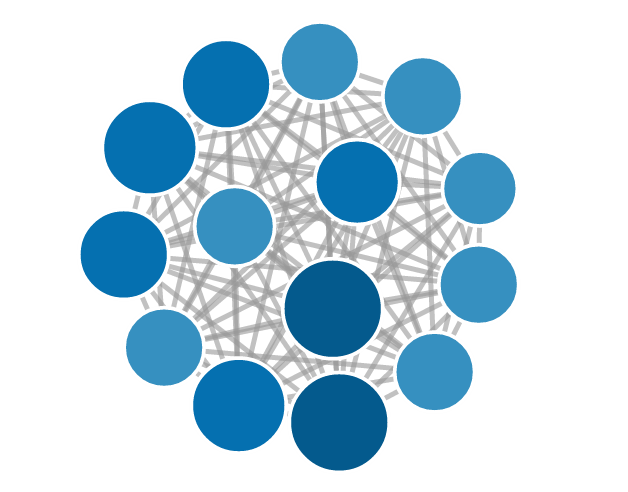
\includegraphics[width=4cm]{Pic3_0.png}
  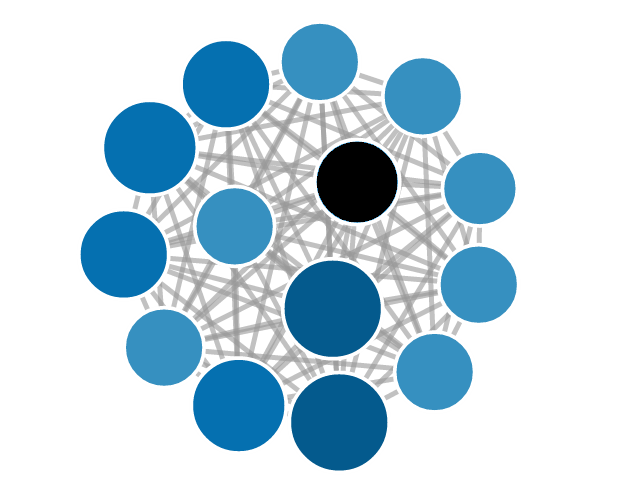
\includegraphics[width=4cm]{Pic3_1.png}
  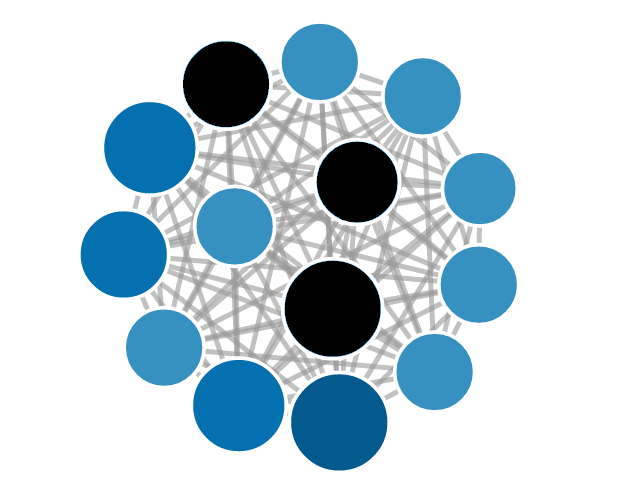
\includegraphics[width=4cm]{Pic3_2.png}
  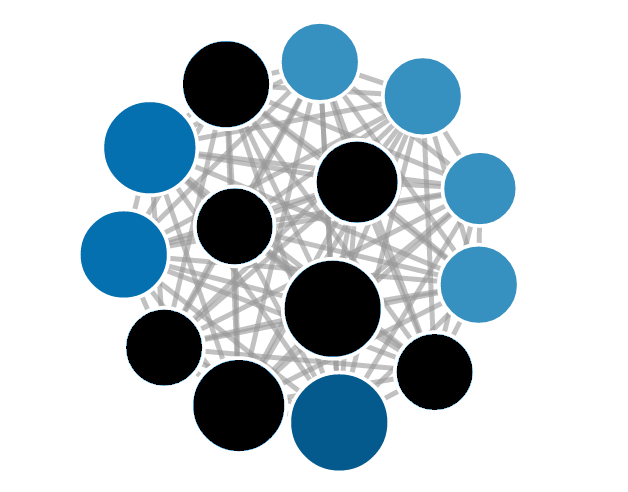
\includegraphics[width=4cm]{Pic3_3.png}
  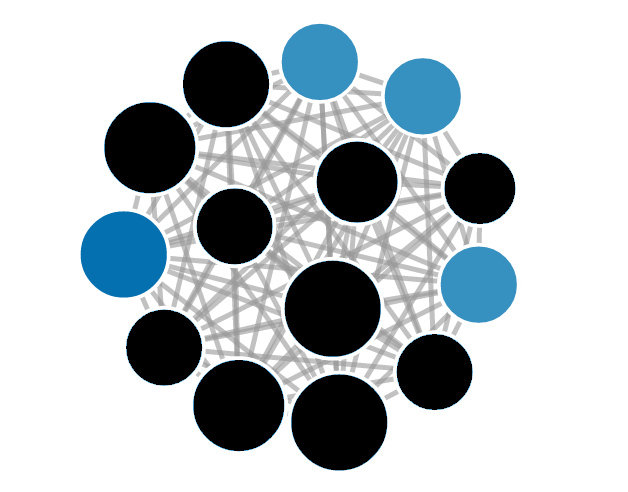
\includegraphics[width=4cm]{Pic3_4.png}
  \caption{Organizational Churn}\label{organizational-churn}
\end{figure}

The black spots in the graph denote employees who have leaved during
the past year. Each graph represents the status of 3 months after the
privious graph. In the first 3 months, there is only one employee leaving the company. In the second 3 months, there are two employees leaving the
company, while 4 more employees leave during the next 3 months. As a
conclusion, there's a phenomenon of organizational churn according to
our model.

\subsection{Productivity}

Firstly, we explain the concept of clustering coefficient [Duncan
J. Watts and Steven Strogatz 1998] of employee indexed by $i$ denoted as $c_{i,t}$, which
is a measure of the degree to which nodes in a graph tend to cluster
together. $c_{i,t}$ is defined as:

\begin{equation}
c_{i,t}=\dfrac{\left| \left\{ s_{jk,t}:v_j,v_k \in M_i,s_{jk,t} \in E
    \right\} \right|}{k_{i,t}(k_{i,t}-1)}
\end{equation}

where
$M_{i,t}=\left\{ v_j:s_{ij,t} \in E \and s_{ji,t} \in E \right\}$ and
$k_{i,t}=\left| N_{i,t} \right|$.

In order to get the definition of productivity, we give some factors
that will influence productivity:

\begin{itemize}
\item The first factor is churn rate which will reduce the
  productivity if churn rate is at a high level.
\item The second factor is the clustering coefficient $c_{i,t}$,
  which determines team cohesiveness. We consider that the higher
  $c_{i,t}$ is, the higher the productivity is.
\item The third factor is the ability of employee indexed by $i$ mentioned in
  \textbf{Section \ref{sec:human-model}}. It is obvious that a higher ability
  brings a higher productivity.
\item The fourth factor is the time duration that
  $i$ stays in his position, denoted as $d_{i,t}$. Productivity will increase as the employee get familiar with his job.
\item The last factor is the salary of employee indexed by $i$, denoed as
  $salary_{i,t}$. It is obvious that salary will influence the productivity.
\end{itemize}

According to the factors described above, we have the formula for calculating productivity:

\begin{equation}
  prod_{i,t}=salary_{i,t} \cdot c_{i,t} \cdot A_{i,t} \cdot d_{i,t} \cdot (1-l_{i,t})
\end{equation}

Finally, we introduce the direct and indirect effects on the
organization's productivity. With the relation updates, edges in our
employee network update, which causes the clustering coefficient
changes. Meanwhile, the salary and work experience will change over
time, which results in the changing of productivity. These factors
effect the productivity collectively.

\section{Further Improved Model}

As the HR manager faces many problems such as identifying employees that
are likely to churn and maximizing employees' knowledge and
abilities, we propose our further improved model to help the HR managers.

\subsection{Incentive Mechanism}
\label{sec:incentive-machanism}

An employee is more likely to churn if he or she was connected to other
former employees who have churned. So there are two kinds of people
who should be highly paid attention to and incented.

Firstly, we should pay attention to those who have more friends than
others. Because of their wide connection with other employees, the
consequence of their churn may be destructive, which can cause many
friends' churn.

Secondly, we focus on those having more friends who have churned
during the past year. This kind of people have a great probability to
churn because of the influence of others.

We choose one sample in our simulations to explain our incentive
mechanism. \textbf{Figure \ref{incentive-mechanism}} shows only 50
people in the sample.

\begin{figure}[htb]
  \centering
  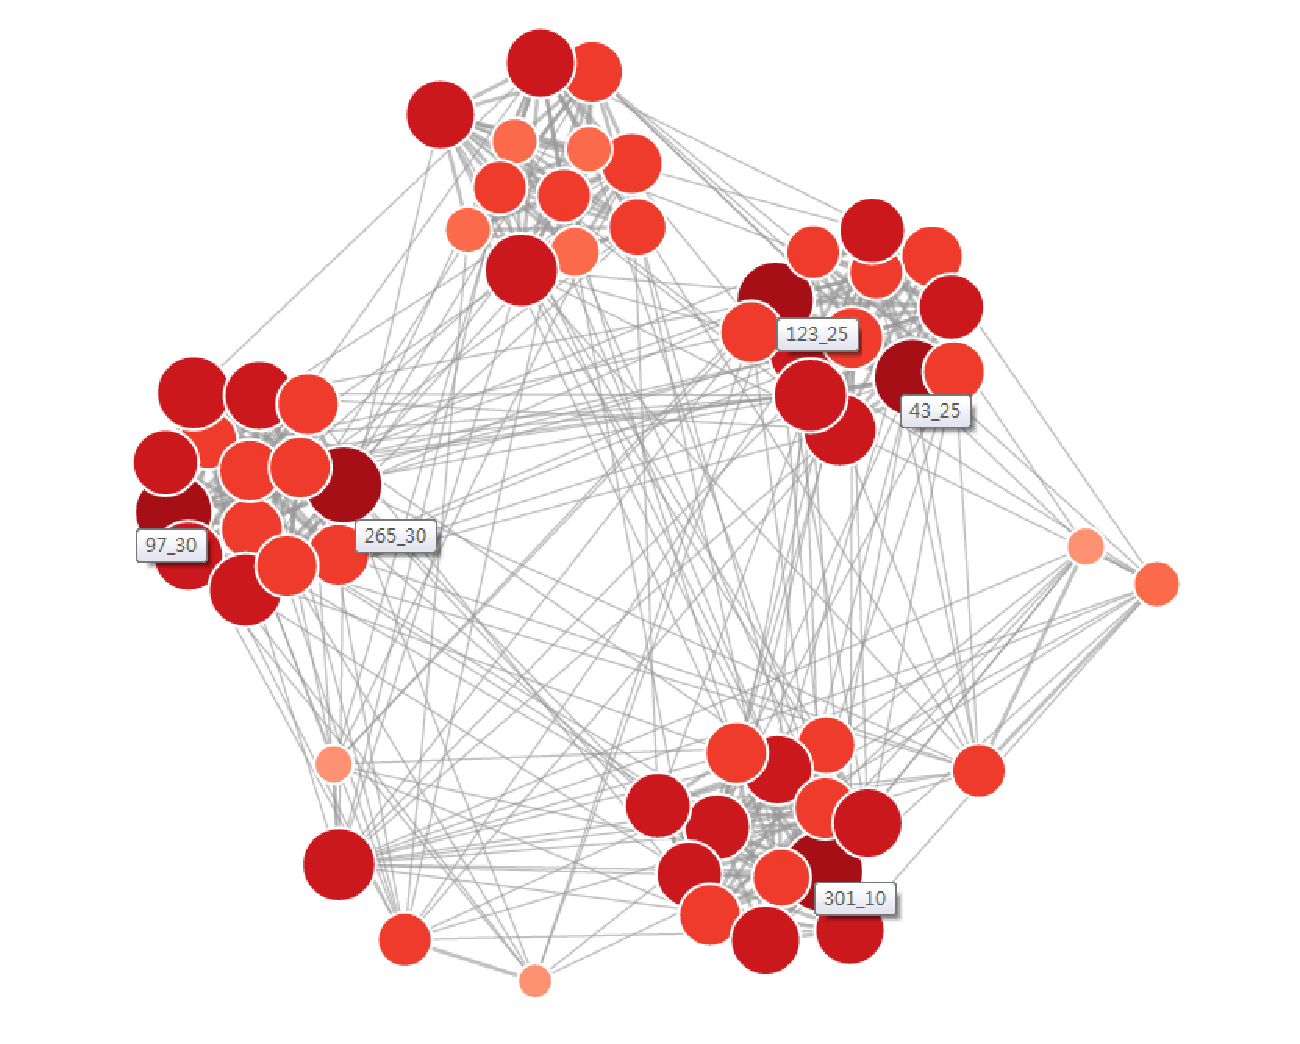
\includegraphics[width=7cm]{p1.eps}
  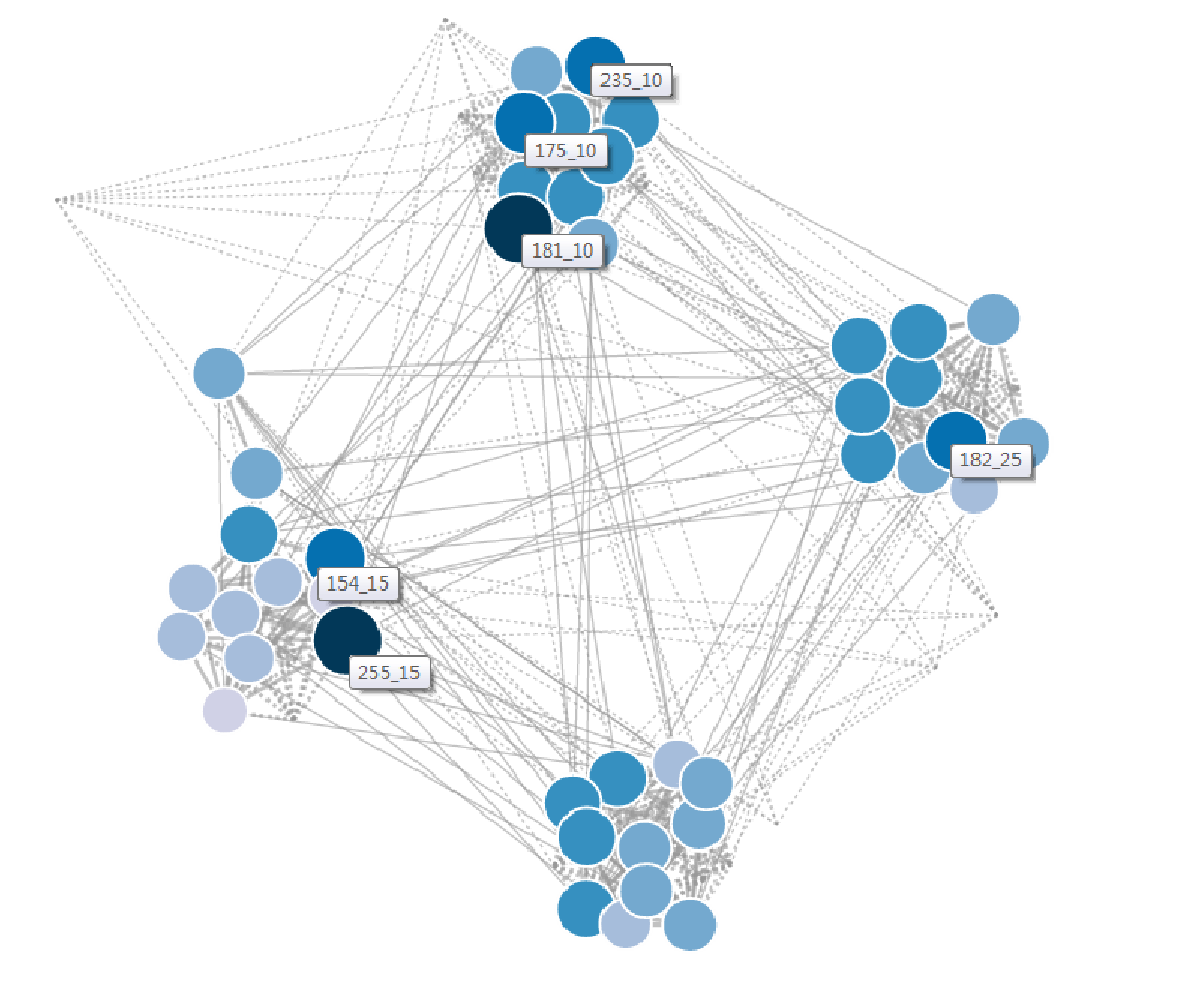
\includegraphics[width=7cm]{p2.eps}
  \caption{Employees should be pay attention
    to}\label{incentive-mechanism}
\end{figure}

In \textbf{Figure\ref{incentive-mechanism}}, as we can see, each vertex
represents an employee, each solid line represents a relation between two
employees, each dotted line represents an relation between a person
who is on the job and a person who have churned. There are 5
employees in left graph we should pay attention to which are employees indexed by 43, 97, 123, 265 and 301 because they have more solid lines than
others. There are 6 employees in the right graph we should pay
attention to which are employees indexed by 154, 175, 181, 182, 235 and 255 because they
have more dotted lines than others.

We should provide incentives to these employees which will decrease their
probabilities to churn.

At $t$-th month, we choose top 10\% of the employees which have the
properties above and reduce their churn rate by 50\%. As shown in
\textbf{Table \ref{churn-rate}}, the churn rate decreases rapidly in one year.

\begin{table}[htb] 
  \centering
  \begin{tabular}{cllllllllllll}
    \toprule[2pt]
    t                          &1&2&3&4&5&6&7&8&9&10&11&12 \\
    \midrule{}
    without incentive mechanism&6&5&7&7&6&6&7&4&5&5&6&6 \\
    with incentive mechanism   &5&3&4&4&4&5&3&3&4&2&4&3 \\
  \bottomrule[2pt]
  \end{tabular}
  \caption{The amount of people leaving}
  \label{churn-rate}
\end{table} 

\subsection{Matching Employees to the Right Positions}
\label{sec:matching-employees-to-the-right-position}

We assume that different employees have different abilities. As we have an
annual evaluation based on performance for each employee and each
division or office has it's necessarily needed abilities, we can match
employees with their most suitable positions.

Because the evaluation is given annually, we reassign employees
annually according to their abilities and the formula below:

\begin{equation}
m_{i,j} =
{(A_{ac_i}-B_{ac_j})}^2 + {(A_{ab_i}-B_{ab_j})}^2 + {(A_{at_i}-B_{at_j})}^2
+ {(A_{po_i}-B_{po_j})}^2
\end{equation}

where $B_{ac_j}$, $B_{ab_j}$, $B_{at_j}$, $B_{po_j}$ represent the
abilities needed for position $j$.

Defining $x_{ij}=\begin{cases} 1 , & \mbox{reassign employee } i
  \mbox{ to position } j \\ 0,&\mbox{otherwise} \end{cases}$, we can
describe this problem as a mathematical programming problem:

\begin{equation}
  \begin{split}
  \min&\sum_{i=1}^n\sum_{j=1}^m m_{ij}x_{ij} \\
  s.t.& \sum_{j=1}^m x_{ij}=1, i=1,2,\ldots,n \\
  &\sum_{i=1}^n x_{ij} \le1,j=1,2,\ldots,m \\
  &x_{ij}=0 \mbox{ or } 1,i=1,2,\ldots,n,j=1,2,\ldots,m
  \end{split}
\end{equation}

We can solve this problem via Kuhn–Munkres algorithm [Harold Kuhn and
James Munkres 1957] whose time complexity is $O(n^4)$.

We reassign them annually according to their
evaluation. \textbf{Figure \ref{reassign}} shows the productivity with reassignment
and without reassignment. We can find that the productivity increases
rapidly after reassigning employees, which means reassignment truly help
with increasing the productivity of the company.

\begin{figure}[htb]
  \centering
  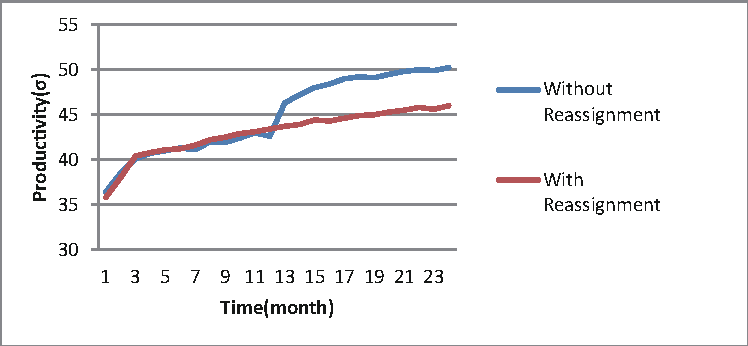
\includegraphics[width=11cm]{p3.pdf}
  \caption{Productivity-Time Curve}\label{reassign}
\end{figure}

\section{Performance and Analysis}
\label{sec:performance-and-analysis}

\subsection{Analysis for Task 3}
\label{sec:analysis-for-task-3}

We assume that the company offers training programs for its employees monthly and newly hired employees start to get their salaries next month after they enter the company. With these two assumptions, results can be drawn according to our model through simulation.

Budget can be divided into threee parts: salary budget, training budget and recruiting budget. The budget requirement predicted for next two years is listed in the \textbf{Table \ref{t3_t} }below in terms of $\sigma$.
\\
\begin{table}[htb]
        \centering
        \begin{tabular}{*{4}{c}}\toprule[2pt]
        Total Budget & Salary Budget & Training Budget & Recruiting Budget\\ \midrule
        1170.8$\sigma$ & 951.387$\sigma$ & 164.423$\sigma$ & 55.08$\sigma$ \\ \bottomrule[2pt]
        \end{tabular}
        \caption{Budget}\label{t3_t}
\end{table}

\subsection{Analysis for Task 4}
\label{sec:analysis-for-task-4}


\begin{figure}[htb]
  \centering
  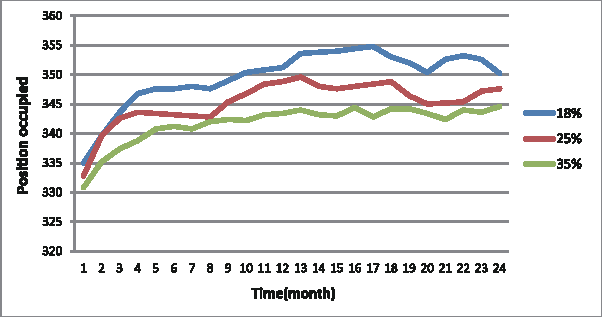
\includegraphics[width=10cm]{task4_p.pdf}\\
  \caption{Status of positions}\label{t4_p}
\end{figure}

To analyze the status of positions under different churn rate, we use
our model to simulate dynamic processes with these churn rate
constraints. We execute our program 100 times for each churn rate and
average the predicted values. \textbf{Figure \ref{t4_p}} shows the averaged
results our model predicted. Under all of these three conditions, the
number of employees in the company keeps rising. The higher the churn
rate, the lower the final full rate the company reaches after two
years. But ICM can sustain its 80\% for positions even if the churn
rate goes to 35\% according to our model's prediction.

\begin{figure}[htb]
  \centering
  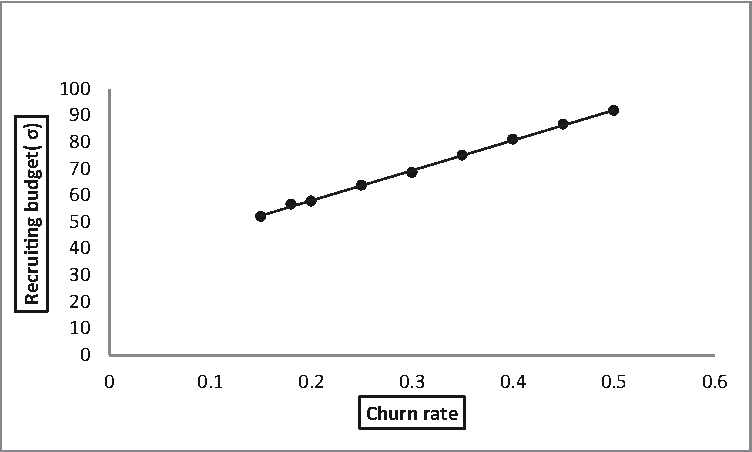
\includegraphics[width=10cm]{task4_r.pdf}\\
  \caption{Recruiting budget}\label{t4_r}
\end{figure}
\begin{figure}[htb]
  \centering
  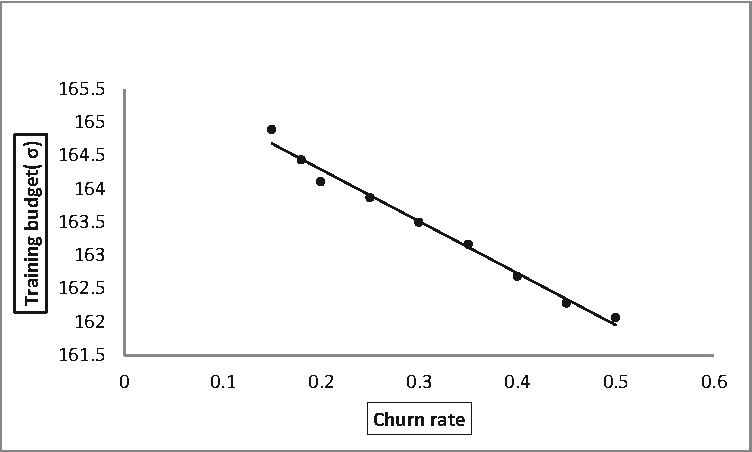
\includegraphics[width=7cm]{task4_t.pdf}
  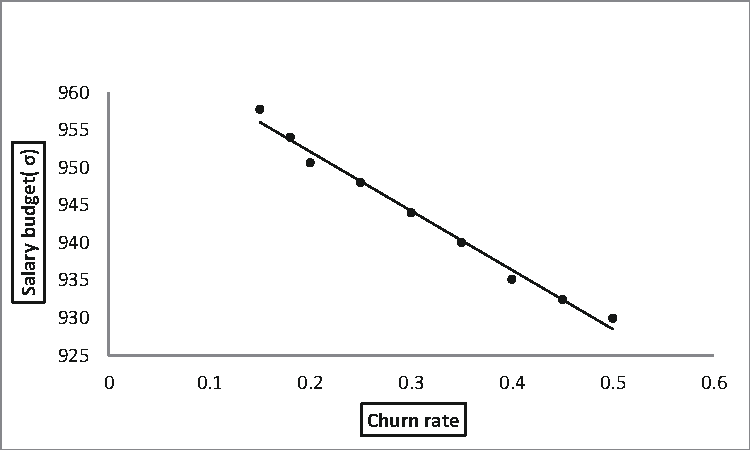
\includegraphics[width=7cm]{task4_s.pdf}\\
  \caption{Training budget and salary budget}\label{t4_t_s}
\end{figure}
The churn rate effects the budget of the company as well. Three
parts of the bugdet behave differently when churn rate increases. The
calculated budget is shown in \textbf{Figure \ref{t4_r}} and \textbf{Figure
\ref{t4_t_s}}. Each data point in three charts is an averaged result of
10 predictions and a linear trendline is added to each chart. It is
clear that recruiting budget showed in \textbf{Figure \ref{t4_r}} is likely to
be proportional to the churn rate while salary budget and training
budget showed in \textbf{Figure \ref{t4_t_s}} are likely to be inversely
proportional to the churn rate.

To maintain enough employees, the company has to spend more on
recruiting. So high turnover rate directly increase the recruiting
budget. High turnover rate's effect on training budget and salary
budget is more complex. On the one hand, when churn rate goes up,
vacancies in the middle level keeps rising due to long recruiting time
and low promotion rate. On the other hand, the vacancies in lower level
rises due to the huge base number. So the full rate of
the company decreases when churn rate rises. Since training budget and
salary budget are closely related to full rate, both of them decrease
when turnover rate goes up.

\subsection{Analysis for Task 5}
\label{sec:analysis-for-task-5}

\begin{figure}[htb]
  \centering
  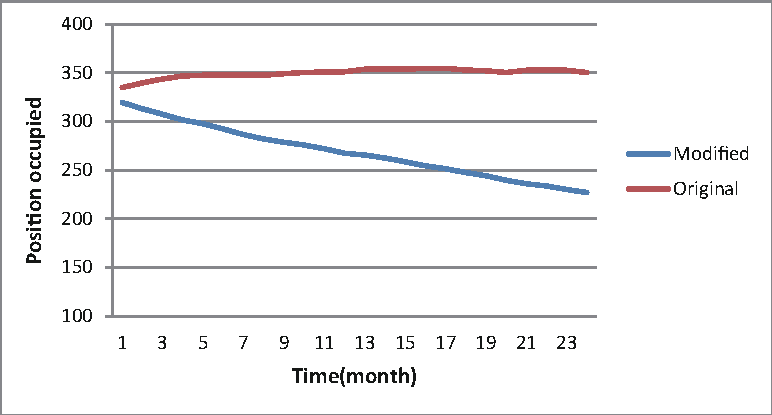
\includegraphics[width=10cm]{task5_p.pdf}\\
  \caption{Status of position}\label{t5_p}
\end{figure}
We apply following changes to our model to simulate the required process:\\
\begin{itemize}
\item Change the churn rate of junior managers and experienced supervisors to 30\%
\item Prohibit external recruiting
\item Promoting only qualified employees
\end{itemize}
\begin{table}
        \begin{center}
                \begin{tabular}{lcc}\toprule[2pt]
                \bfseries Level of Position & \bfseries Modified & \bfseries Original\\ \midrule
                Senior manager/Executive & 5.6 & 8.4\\
                Junior manager/Executive & 9.0 & 18.4\\
                Experienced supervisor & 7.4 & 23.0\\
                Inexperienced supervisor & 9.2 & 23.2\\
                Experienced employee & 72.6 & 107.4\\
                Inexperienced employee & 99.6 & 149.6\\
                Administrative clerk & 24.0 & 24.0\\ \bottomrule[2pt]
                \end{tabular}
                \caption{Status of position}\label{t5_p_t}
        \end{center}
\end{table}

The result of simulation is shown in \textbf{Figure \ref{t5_p}} and \textbf{Table
\ref{t5_p_t}}. All the data shown is an average of ten
predictions. While the number of positions occupied remains stable
with origial conditions, it drops remarkably with modified
conditions.

We list specific data of each level in \textbf{Table \ref{t5_p_t}}. In the
modified case, the numbers of employees are lower than original case
especially those of the middle levels. Since there is no external
recruiting in modified case, it is obivious that the full rate will
decrease due to employees' leave. Although some qualified employees
can be promoted into higher level, the high churn rate of the middle
level and difficulty of satisfying the promotion conditions make the
numbers of middle level employees relatively low. The situation given
in task 5 will cause unrecoverable damage to ICM's HR
health. With the full rate of middle level employees lower than 50\%,
the HR structure is broken into fragments and the company won't be
able to function normally.

\section{Team Science and Multi-layered Network}
\label{sec:team-science}
This part summarizes the potential use of team science and multi-layered networks in this problem.

Team Science shows how team works with team and how team members
intereffect. The theory is helpful for promoting team cohesiveness and
teamwork effeciency. The existing researches suggest that an
organization aiming to improve its teamwork effeciency should establish its team
cognition, evaluate the individuals appropriately, provide team
training and try to identify the factors that influence the team performance\cite{8}\cite{9}.

A well-designed model can be great helpful to achieve goals listed above. Multi-layered model is a good example. We will introduce how to connect our model to the other organizational network
layers such as information flow, trust, influence and
friendship. Number the layers from 0 to
k. $$G^\alpha=(V^\alpha,E^\alpha), \alpha=1,2,\ldots,k$$ Each
$E^\alpha$ is colored by a specific color. $G^0$ reprensents the
network we built before, $G^1, G^2, \ldots ,G^k$ represent the other layers added.

Still, in each network layer $G_\alpha$, $N_i$ represents employee
$i$. The edge $e_{ij}$ connects between two nodes $N_i$ and
$N_j$. Each edge has a value $w_{ij}^\alpha$ proving the weight of
edge $e_{ij}^\alpha$, positive correlated to the strength of
connection between two employees in network layers $\alpha$. Then we
connect these network layers together to built a general network
$G_e=(V, E, C)$, V is node set, C is color set, $E\subset V\times
V\times C$ is edge set\cite{10}. In the general model, different layers effect
each other. Take an example, if the friendship between employee indexed by $i$
and employee indexed by $j$ is deeper, with other conditions same, their
information flow will be more fluent. $w_{ij}^\alpha$ is changing with time
flows and $G_e$ is a dynamic network.

However, the human capital network plays a leading role to other network layers. In the general network, if an empolyee churns or is
reassigned, the edge related to him will change. That is,
$w_{ij}^\alpha$ get a new value for all $\alpha$. Hence, human capital
network takes the lead in this effort.

\section{Sensitivity Analysis}
\label{sec:sensitivity-analysis}

We analyze sensitivity of our model by running the program with modified parameters. The results are shown in \textbf{Table \ref{sensi}}.
\begin{table}[htb]
\begin{tabular}{cccccccc}\toprule[2pt]
\thead{Parameter}    &\thead{Variation}           &\thead{N}                    &\thead{p}             &\thead{Training\\ Budget}       &   \thead{Salary\\ Budget}   &  \thead{Recruit\\ Budget}     &\thead{Total\\ Budget}     \\
\hline r & +5\%        &0\%                  & +1.3\%       &+0.46\% &+0.6\% & -0.49\% &+0.5\%     \\
                    & -5\%        &+0.8\%               & -4\%         &-3.5\%  &-4.4\% & -8.5\%  &+4.5\%     \\
\hline c   & +5\%        &-1.4\%               & -2.1\%       &-0.2\%  &-0.5\% &+12.4\%  &+0.1\%    \\
                    & -5\%        &0\%                  & +1.1\%       &0.4\%   &+0.7\% &-11.7\%  &+0.1\%    \\
\hline ra        & +1          &-0.9\%               & -0.6\%       &-1.2\%  &-1.7\% &+24.0\%  &-0.5\%   \\
                    & -1          &+1.1\%               & +6.7\%       &+1.0\%  &+0.8\% &-17.4\%  &-0.1\%      \\ \bottomrule[2pt]
\end{tabular}
\caption{Sensitivity analysis}\label{sensi}
\end{table}

With $c$ rising, $N$ and $p$ keeps stable. When $c$ drops, they varies
more clearly. It is because in current condition, the positions are
nearly all occupied. It won't make obvious change if $c$ rises. For
the similar reason, $N$ and $p$ changes little when $c$ drops while
they changes more clearly when $c$ increases. If $ra$ drops to 1, $N$
and $p$ increase considerably, which proves that reducing middle
manangers' churn rate is quite beneficial to HR health. As for the budget
requirements, training budget, salary budget and total budget stay
stable, while recruiting budget changes quite obviously. It is because
the change of these paramenters greatly changed the number of the
newly-recruited employees. The other budgets change relatively lower
because they are mainly associated to $N$, which doesn't change much
while $ra$ varies.

\section{Strengths and Weaknesses}
\label{sec:strengths-and-weaknesses}

\subsection*{Strengths}
\label{sec:strengths}

\begin{itemize}
\item Our model make full use of the theory of multilayer networks so
  that it quantizes the relation accurately and reasonablly.
\item Our model exellently proves the interaction among these
  factors: leave probability, promotion probability and productivity.
\item The network we built includes both microcosmic and macrocosmic which react to each other.
\item Our model is robust according to sensitivity test.
\end{itemize}

\subsection*{Weaknesses}
\label{sec:weaknesses}

\begin{itemize}
\item Limited by the time, we neglected sorts of factors which are not
  so significant. In fact, the model still has space to be perfected.
\item Our result involves some randomness.
\end{itemize}

\section{Conclusions}
\label{sec:conclusions}

For Task 1, we propose an Employee Relation Model based on the SNA
(social network analysis) technique. Meanwhile each node (employee) in
the network has several characteristics which are used to evaluate the
employee corresponding to the node. We calculate the grade of each
employee by evaluating based on AHP (analytic hierarchy process)
technique. Based on these grades, we predict the promotion probability
for each employee in the company.

For Task 2, we establish an Organizational Churn Model to simulate the
effects caused by the leaving of employees. Furthermore, we introduce
a new method to calculate the productivity considering five factors,
including churn rate, team cohesiveness, employee ability, work
experience and salary.

For Task 3 and 4, we calculate the budget for the next two years and
analyze the influence of different churn rates. Our data show that the
cost of recruitment increases, while the cost of training and salary
decreases when the churn rate rises.

For Task 5, we simulate the situation which doesn't have external
recruitment, and get the result that the amount of employees decreases
rapidly.

For Task 6, we discuss the potential usage of team science and
multi-layered network and apply them into our model.

Moreover, we propose an improved version of our model which can
analyze the influence of reassignment and provide reference value to
HR managers for incentive mechanism.

% the reference
\begin{thebibliography}{99}


\bibitem{1} Huang Y. A Study of the Performance Assessment of State-owned Power Enterprisees[D]. Tianjing University, 2010.

\bibitem{2} Journal T E D O T. The Investigation Report of the Condition of employee churn in 2011[J]. China New Time, 2012(2).

\bibitem{3} Zhang J. The Empirical Research of the Factors effecting employee churn in Resource-oriented Enterprise in Yuncheng,Shandong [D]. Southerneast University, 2014.

\bibitem{4} J.A.Alonso and M.T.Lamata, Consistency in the Analytic Hierarchy Process: A New Approach, International Journal of Uncertainty, Fuzziness and Knowledge-Based Systems, Vol.14, No.4, 2006.

\bibitem{5} MEJNewman. The Structure and Function of Complex Networks[D]. University of Michigan, 2003.

\bibitem{6} Fang J, Zheng Z, Bi Q, etal. A Brand-new
Interdisciplinary Science: Network Science (Part One)[J]. Progress in Physics, 2007, 27(3).

\bibitem{7} Fang J, Zheng Z, Bi Q, etal. A Brand-new
Interdisciplinary Science: Network Science (Part Two)[J]. Progress in Physics, 2007, 27(4).

\bibitem{8} E. Salas, N.J. Cooke, and M.A. Rosen. (2008). On Teams, Teamwork, and Team Performance: Discoveries and Developments. Human Factors: The Journal of the Human Factors and Ergonomics Society June 2008 vol. 50 no. 3540-547.

\bibitem{9} D. Stokols, K.L. Hall, B.K. Taylor, R.P. Moser (2008). The Science of Team Science: Overview of the Field and Introduction to the Supplement, Am J Prev Med 2008;35(2S): S77-S89.

\bibitem{10} Mikko Kivelä, Alexandre Arenas, Marc Barthelemy, James P. Gleeson, Yamir Moreno, Mason A. Porter. (2013). Multilayer Networks, J. Complex Networks, 2(3): 203-271 (2014); arXiv preprint arXiv:1309.7233, 2013.

\bibitem{11} Saaty, Thomas L. Decision making with the analytic hierarchy process. International Journal of Service Sciences. 2008, 1: 83–98.

\end{thebibliography}

\label{LastPage}

\end{document}

%%% Local Variables:
%%% mode: latex
%%% TeX-master: t
%%% End:
